\documentclass{article}

% if you need to pass options to natbib, use, e.g.:
%     \PassOptionsToPackage{numbers, compress}{natbib}
% before loading neurips_2023

% ready for submission
\usepackage[final]{neurips_2023}

% to avoid loading the natbib package, add option nonatbib:
%    \usepackage[nonatbib]{neurips_2023}

\usepackage[utf8]{inputenc} % allow utf-8 input
\usepackage[T1]{fontenc}    % use 8-bit T1 fonts
\usepackage{hyperref}       % hyperlinks
\usepackage{url}            % simple URL typesetting
\usepackage{booktabs}       % professional-quality tables
\usepackage{amsfonts}       % blackboard math symbols
\usepackage{amssymb}        % for math symbols like \leq and \geq
\usepackage{nicefrac}       % compact symbols for 1/2, etc.
\usepackage{microtype}      % microtypography
\usepackage{xcolor}         % colors
\usepackage{graphicx}       % for including figures
\usepackage{subcaption}     % for subfigures
\usepackage{float}          % for H placement option

\title{MLPC 2025: Sound Event Detection Data Exploration}

\author{
  Team Imported \AND
  Lóránd Heidrich
  \And
  Mark Sere
  \And 
  Gergely Terényi
  \And 
  Diego Caparros Vaquer
}

\begin{document}

\maketitle

\begin{abstract}
This report presents our exploratory data analysis of the MLPC 2025 Sound Event Detection dataset. We investigate annotation quality, audio feature characteristics, and text feature patterns to understand the dataset's suitability for training general-purpose sound event detection systems. Our analysis quantifies temporal precision and textual similarity of annotations, identifies the most important audio features through dimensionality reduction, and examines clustering patterns in both audio and text features. The findings help identify potential challenges and biases in the dataset, providing valuable insights for subsequent model development phases.
\end{abstract}

\section{Introduction}

This report presents our data exploration analysis for the MLPC 2025 Sound Event Detection dataset. Kepler Intelligent Audio Labs (KIAL) has collected a dataset of audio recordings with free-text annotations for training sound event detection systems. Our analysis investigates various aspects of this dataset, including annotation quality, audio features, and text features, to understand its characteristics and potential challenges for further processing.

The dataset consists of 9,026 audio files annotated by 330 students, containing 35,826 textual annotations. Each audio file is between 15 to 30 seconds long, with at least one annotation per file and four on average. The annotations include textual descriptions of sound events along with their temporal onsets and offsets.

\section{Case Study}
\label{sec:case_study}

\subsection{Temporal & Textual Annotation Comparison}
Audio 1 (407115.mp3):

Temporal Overlap:

All annotators agree on a long segment (0–29s) containing multiple events.

Annotators 2 and 3 both highlight sound events between ~16s and 22s (honking, beeping, scratching).

Differences in segment precision — Annotator 1 uses broader intervals, while Annotators 2 & 3 mark finer-grained events.

Textual Similarity & Differences:

All three detect people talking — described as “lively crowd,” “people talking,” and “somebody sweeping” (possibly mistaken interpretation).

Annotators 2 & 3 label overlapping sound events like honks or beeps, but use slightly different language ("horn honking", "a honking sound", "a beeping sound").

Annotator 2 uniquely identifies a sewing machine and wheel scratching, indicating higher event resolution or different interpretation.

Audio 2 (352781.mp3):

Temporal Annotations (Onset/Offset)

High agreement across annotators on the full duration of the audio (approx. 0 to 16.4s).

Small differences in onset (e.g., 0.0 vs. 0.028 or 0.056) are minimal and likely due to human precision.

All annotators treat the clip as a continuous ambient scene rather than short, isolated events.

Similarities:

All three annotators identify:

Human speech: Described as "muffled", "unclear", "multiple people"

Background noise: Captured as "white noise", "engine", "hum"

All are describing a confined indoor-like sound environment (e.g., inside a bus or a room)

Differences:

A1 explicitly identifies the context ("on a bus")

A2 generalizes to "close space" and "white noise"

A3 adds more detail, identifying a radio and engine with specific qualifiers ("silently", "evenly indoors")

\subsection{Deviation from keywords and textual descriptions in the
audio’s metadata}

407115.mp3

Matches / Reliance : "people talking", "lively crowd" → matches people, market, mall

"sewing machine noise" → directly reflects sewing, machines, textile

Deviations / Additions:

"horn honking", "beeping", "wheel scratching" → Not present in keywords

These are foreground events perceived by annotators but not described in metadata

Conclusion:

Annotations rely heavily on keywords for background context (people, sewing, market scene)

Annotators go beyond the metadata by identifying short, foreground sound events (e.g., honks)

352781.mp3

Matches / Reliance:

"engine of a heavy vehicle", "bus driving" → matches engine, bus, vehicle

"people speaking", "voices", "talking" → matches people, voices, talking

"radio playing" → directly matches radio

"white noise", "ambience" → aligns with ambience

Deviations / Additions:

Very few! Maybe "white noise" adds a perceptual detail, but it’s covered by ambience

Conclusion:

This is a textbook example of alignment

Annotations match nearly all metadata keywords, showing strong reliance and task alignment

\subsection{Done according to task description?}

For 407115.mp3 (Urban Environment with Crowd and Sewing Sounds)

Temporal Annotation Compliance:

Onset and Offset: The annotators followed the rule of annotating distinct sounds. For example:

People talking: Different annotators split the crowd noise into multiple events (e.g., a continuous sound, then specific people talking). The annotations' onset/offset reflects this continuous nature of the sound, as suggested by the task (e.g., "people talking" marked over a longer period).

Sewing machine: This was marked as a continuous sound with an onset at the start and an offset at the end of the sound.

Honking, beeping, and wheel scratching: These are separate events, as per the task's rule of separating events when noticeable pauses are present. Annotators made distinct annotations for each.

The temporal boundaries are consistent and correct based on the task's example. For instance, the “sewing machine noise” annotation lasts throughout the segment where the machine sound is heard, fitting the continuous sound rule.

Textual Annotation Compliance:

Specific Descriptions: The descriptions follow the task’s required level of detail:

Source and Action: Each annotation specifies the source of the sound (e.g., "sewing machine noise," "people talking").

Descriptor: Descriptions like "lively," "muffled," and "tonal" provide insight into how the sounds were perceived.

Context: Annotators provide an environmental context where relevant (e.g., “crowd outdoors,” “in the background,” “indoors”).

The annotations adhere to the one description for one sound rule (e.g., separate descriptions for "honking," "wheel scratching," and "people talking").

Conclusion:

The temporal and textual annotations are fully compliant with the task description. The annotators correctly followed guidelines for separating sounds, providing detailed annotations, and aligning their work with the task’s structure.

For 352781.mp3 (Bus Environment with People Talking and Engine Sounds)

Temporal Annotation Compliance:

Onset and Offset: The annotators marked the entire recording as a single region for continuous sounds like engine hum and ambient voices, which aligns with the continuous sound rule (e.g., "low hum of a bus driving steadily").

In contrast, short events like horn honking or radio playing were marked separately, showing the annotators correctly handled short, separate sound events and gaps in between.

The temporal boundaries for each sound event are appropriate, and the overlapping sounds (e.g., bus engine and talking) are managed correctly.

Textual Annotation Compliance:

Specific Descriptions: The descriptions follow the task’s rule of detailed annotations:

Source and Action: Each annotation specifies the source of the sound (e.g., "engine of a heavy vehicle," "voices of people").

Descriptor: Descriptions like “hissing,” “soft,” and “muffled” describe how the sound was perceived.

Context: The context is well-defined, with mentions of "indoors," "in the distance," and "close by."

No multiple events are described in a single annotation, meaning each description corresponds to one sound event.

Conclusion:

The temporal and textual annotations for this recording are also fully compliant with the task description. Annotators successfully separated distinct sounds, followed the rules for continuous versus discrete events, and provided detailed textual descriptions.

\section{Annotation Quality}
\label{sec:annotation_quality}

\subsection{Temporal Annotation Precision}

Temporal annotation precision was evaluated by comparing the onset and offset timings of overlapping regions from different annotators on the same audio file, considering only segments where a temporal overlap was present. The key metrics were Euclidean distance, onset and offset differences, and their means.

\begin{figure}[H]
  \centering
  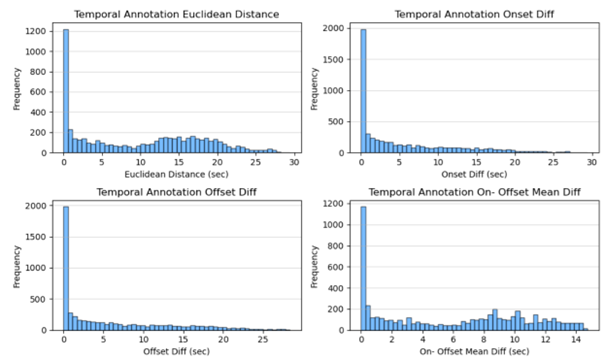
\includegraphics[width=0.8\textwidth]{figures/annotation_quality/temporal_annotation_differences.png}
  \caption{Temporal Annotation Differences}
  \label{fig:temporal_diff}
\end{figure}

The results show a distinct spike around 0 sec, meaning the majority of annotators strongly agree on start and end times. All four distributions show a long positive skew. While the onset and offset distributions show consistent gradual decay starting before the 5 second mark, the Euclidean distance analysis highlights a secondary hump in the 12-20 second range, indicating a stronger disagreement pattern here.

The results point to high general temporal precision, however, a significant amount of annotations do differ in timing, pointing to possible ambiguity in some of the audio that makes it harder to segment.

\subsection{Text Annotation Similarity}

\begin{table}[H]
  \caption{Similarity of Overlapping Text Annotations Stats}
  \label{tab:text_similarity}
  \centering
  \begin{tabular}{lc}
    \toprule
    Metric & Value \\
    \midrule
    Range & -0.29 -- 0.75 \\
    Mean & 0.088 \\
    Median & 0.072 \\
    \bottomrule
  \end{tabular}
\end{table}

Most overlapping annotations show low textual similarity across different annotators. The cosine similarities ranges from -0.29 -- 0.75, with a mean of 0.088 and a median of 0.072, indicating that many annotators differ in their wording or focus (see Table~\ref{tab:text_similarity}). The histogram confirms this by showing a concentration of values between 0 and 0.2, suggesting generally weak agreement in textual descriptions even when annotators mark the same time span.

\begin{figure}[H]
  \centering
  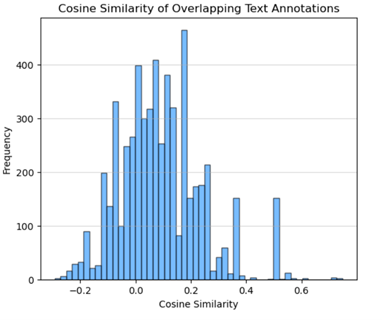
\includegraphics[width=0.8\textwidth]{figures/annotation_quality/similarity_of_overlapping_text_annotations.png}
  \caption{Similarity of Overlapping Text Annotations}
  \label{fig:text_similarity}
\end{figure}

\subsection{Annotation Distribution}

\begin{table}[H]
  \caption{Per File Measures}
  \label{tab:per_file}
  \centering
  \begin{tabular}{lcc}
    \toprule
    & Annotations/File & Distinct Sound Events/File \\
    \midrule
    Total Unique Files & 9026 & 9026 \\
    Total Annotations & 35826 & 35826 \\
    Mean & 3.9692 & 2.4253 \\
    Median & 2 & 2 \\
    STD & 4.4254 & 1.9063 \\
    Min & 1 & 1 \\
    Q1 & 1 & 1 \\
    Q2 & 2 & 2 \\
    Q3 & 5 & 3 \\
    Max & 96 & 27 \\
    \bottomrule
  \end{tabular}
\end{table}

Table~\ref{tab:per_file} shows the statistics for annotations per file and distinct sound events per file. The dataset has a mean of approximately 4 annotations per file with a median of 2, indicating a positively skewed distribution. The maximum number of annotations for a single file is 96, which is significantly higher than the average.

\begin{figure}[H]
  \centering
  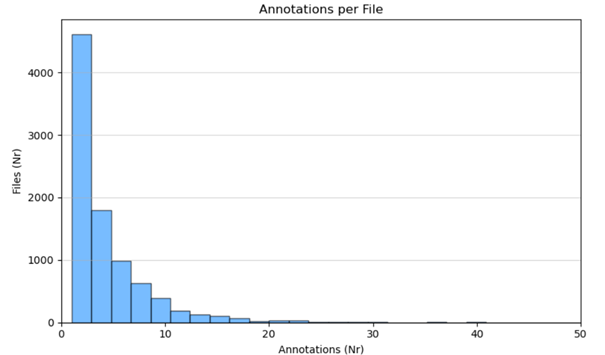
\includegraphics[width=0.8\textwidth]{figures/annotation_quality/annotations_per_file.png}
  \caption{Annotations Per File}
  \label{fig:annotations_per_file}
\end{figure}

\begin{figure}[H]
  \centering
  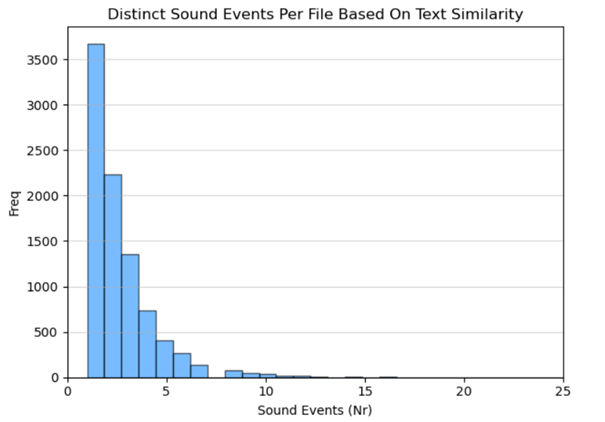
\includegraphics[width=0.8\textwidth]{figures/annotation_quality/distinct_sound_events_per_file.png}
  \caption{Distinct Sound Events Per File}
  \label{fig:events_per_file}
\end{figure}

\subsection{Annotation Detail and Quality Variation}

\begin{table}[H]
  \caption{Text Annotation Detail}
  \label{tab:text_detail}
  \centering
  \begin{tabular}{lc}
    \toprule
    Metric & Value \\
    \midrule
    Total annotations & 35826 \\
    Mean word count & 7.4874 \\
    Median & 7 \\
    STD & 4.6315 \\
    Min & 1 \\
    Q1 & 4 \\
    Q2 & 7 \\
    Q3 & 9 \\
    Max & 88 \\
    \bottomrule
  \end{tabular}
\end{table}

The annotations have an average word count of 7.85 words. The histogram in Figure~\ref{fig:word_count} shows a concentration between 5-10 words (a reasonable amount considering the annotation guidelines), however some annotators averaged over 20 words. The positive skew is indicative of this high variability.

\begin{figure}[H]
  \centering
  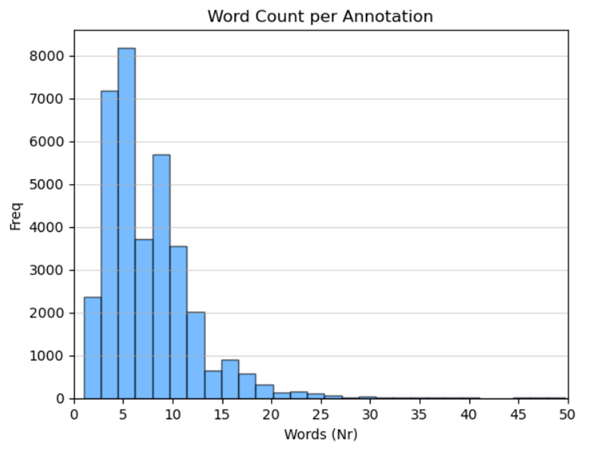
\includegraphics[width=0.8\textwidth]{figures/annotation_quality/word_count_per_annotation.png}
  \caption{Word Count Per Annotation}
  \label{fig:word_count}
\end{figure}

\begin{figure}[H]
  \centering
  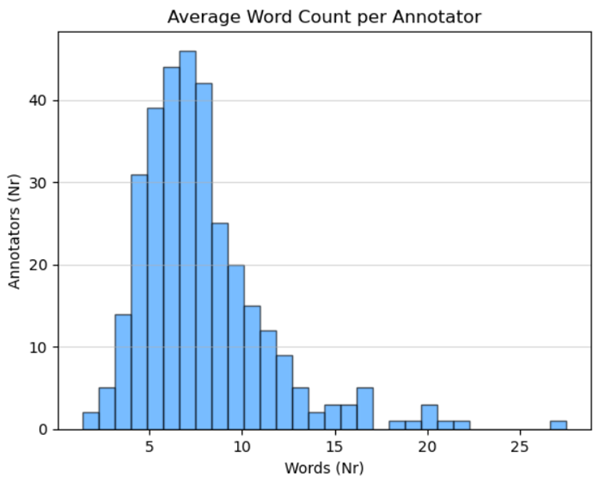
\includegraphics[width=0.8\textwidth]{figures/annotation_quality/average_word_count_per_annotator.png}
  \caption{Average Word Count Per Annotator}
  \label{fig:avg_word_count}
\end{figure}

Most annotators marked events lasting in the 5-10 second range, with an overall average of 8.38 sec. The distribution's long tail indicates some annotators consistently marked longer events, ranging over 20 seconds, indicating a difference in how annotators perceive events. The standard deviation of 3.31 seconds indicates moderate variation in the average durations used by different annotators.

\begin{figure}[H]
  \centering
  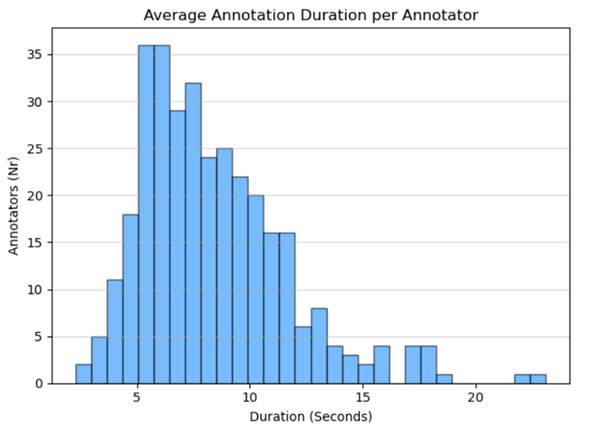
\includegraphics[width=0.8\textwidth]{figures/annotation_quality/average_annotation_duration_per_annotator.png}
  \caption{Average Annotation Duration Per Annotator}
  \label{fig:avg_duration}
\end{figure}

\subsection{Inconsistencies and Quality Issues}

Annotation duration, word count, and spelling errors were the indicators used to detect inconsistencies, outliers, and poor-quality annotations. Outlier thresholds were set both by IQR and explicit selection, following best practices and empirical testing.

\begin{table}[H]
  \caption{Duration and Word Count Metrics}
  \label{tab:duration_word}
  \centering
  \begin{tabular}{lcc}
    \toprule
    & Duration & Word Count \\
    \midrule
    Count & 35826 & 35826 \\
    Mean & 7.3139 & 7.4874 \\
    Median & 2.6609 & 7 \\
    STD & 8.7611 & 4.6315 \\
    Min & 0 & 1 \\
    1\% & 0.1323 & 2 \\
    5\% & 0.2721 & 2 \\
    Q1 & 0.9712 & 4 \\
    Q3 & 12.6279 & 9 \\
    95\% & 26.1306 & - \\
    99\% & 29.2635 & - \\
    Max & 30.0447 & 88 \\
    IQR & 11.6567 & 5 \\
    IQR lower threshold & -16.5138 & -3.5 \\
    IQR upper threshold & 30.113 & - \\
    \bottomrule
  \end{tabular}
\end{table}

Event duration markers found no IQR lower outliers, therefore the central range is wide and tolerant. Explicit 1\%/99\% thresholds flagged 0.99\%/1\% of annotations respectively, while 5\%/95\% thresholds flagged 5\% each, showing that most annotations are reasonable, with few consistent outliers.

\begin{table}[H]
  \caption{Duration Outcomes}
  \label{tab:duration_outcomes}
  \centering
  \begin{tabular}{lccc}
    \toprule
    & IQR & 99\% & 95\% \\
    \midrule
    Text too short (annotations) & 0 & 355 & 1792 \\
    Text too long (annotations) & 0 & 359 & 1792 \\
    Text too short (\%) & 0\% & 0.9909\% & 5.0020\% \\
    Text too long (\%) & 0\% & 1.0021\% & 5.0020\% \\
    \bottomrule
  \end{tabular}
\end{table}

Text description length, identified by word counts per annotation also found no lower outliers by IQR threshold. Percentile thresholds flagged 0.94\% of annotations under the fifth percentile. Explicit counts found no zero-word annotations, 335 one-word, 2024 two-word, and 3146 three-word annotations. A total of 9537 annotations, marking 26.62\% of the population were under the five-word threshold, arbitrarily found to be ideal for describing annotations based on the guidelines, potentially marking a large portion of the population as poor.

\begin{table}[H]
  \caption{Word Count Outcomes}
  \label{tab:word_outcomes}
  \centering
  \begin{tabular}{lcccc}
    \toprule
    & 1\% & 5\% & IQR Lower & Explicit 5 \\
    \midrule
    Word threshold & 2 & 2 & -3.5 & 5 \\
    Annotation Count & 335 & 335 & 0 & 9537 \\
    Annotation Proportion & 0.9351\% & 0.9351\% & 0\% & 26.6203\% \\
    \bottomrule
  \end{tabular}
\end{table}

Spelling was measured with Python's pyspellchecker module to gauge effort and commitment to the task. 49.56\% of annotations had no spelling errors. 32.3\% had one misspelled word, nearly 15\% had 2-3 misspelled words, leaving around 3\% with 4 or more misspelled words.

Combining all three criteria, with duration (below 1\% or above 99\%), short text ($\leq$ 2 word count), and a high misspell count ($\geq$ 3), 15.25\% of annotations were flagged as having poor quality. Using a 5\% duration threshold raised this to 22.14\%.

It is important to note that after filtering for files with multiple annotators, each annotator has on average annotated only 4.5 files with a STD of 2.59 files. A minimum and maximum of 1 and 27 respectively are indicative of a positive skew, and an overall small dataset that may provide inconclusive results.

\subsubsection{Proposed Solution for Inconsistencies}

Spelling errors can be fixed programmatically, flagging the annotation for review. Word count and duration outliers can be flagged in the same manner. A random sample of this subset will reveal the possible necessity of reannotating these flagged files. If necessary, the group of files can be reassigned to their respective annotators.

\section{Audio Features}
\label{sec:audio_features}

\subsection{Feature Selection and Dimensionality Reduction}

Given the high dimensionality of the feature space (942 dimensions), Principal Component Analysis (PCA) was applied to reduce dimensionality while preserving the most important information.

\begin{figure}[H]
  \centering
  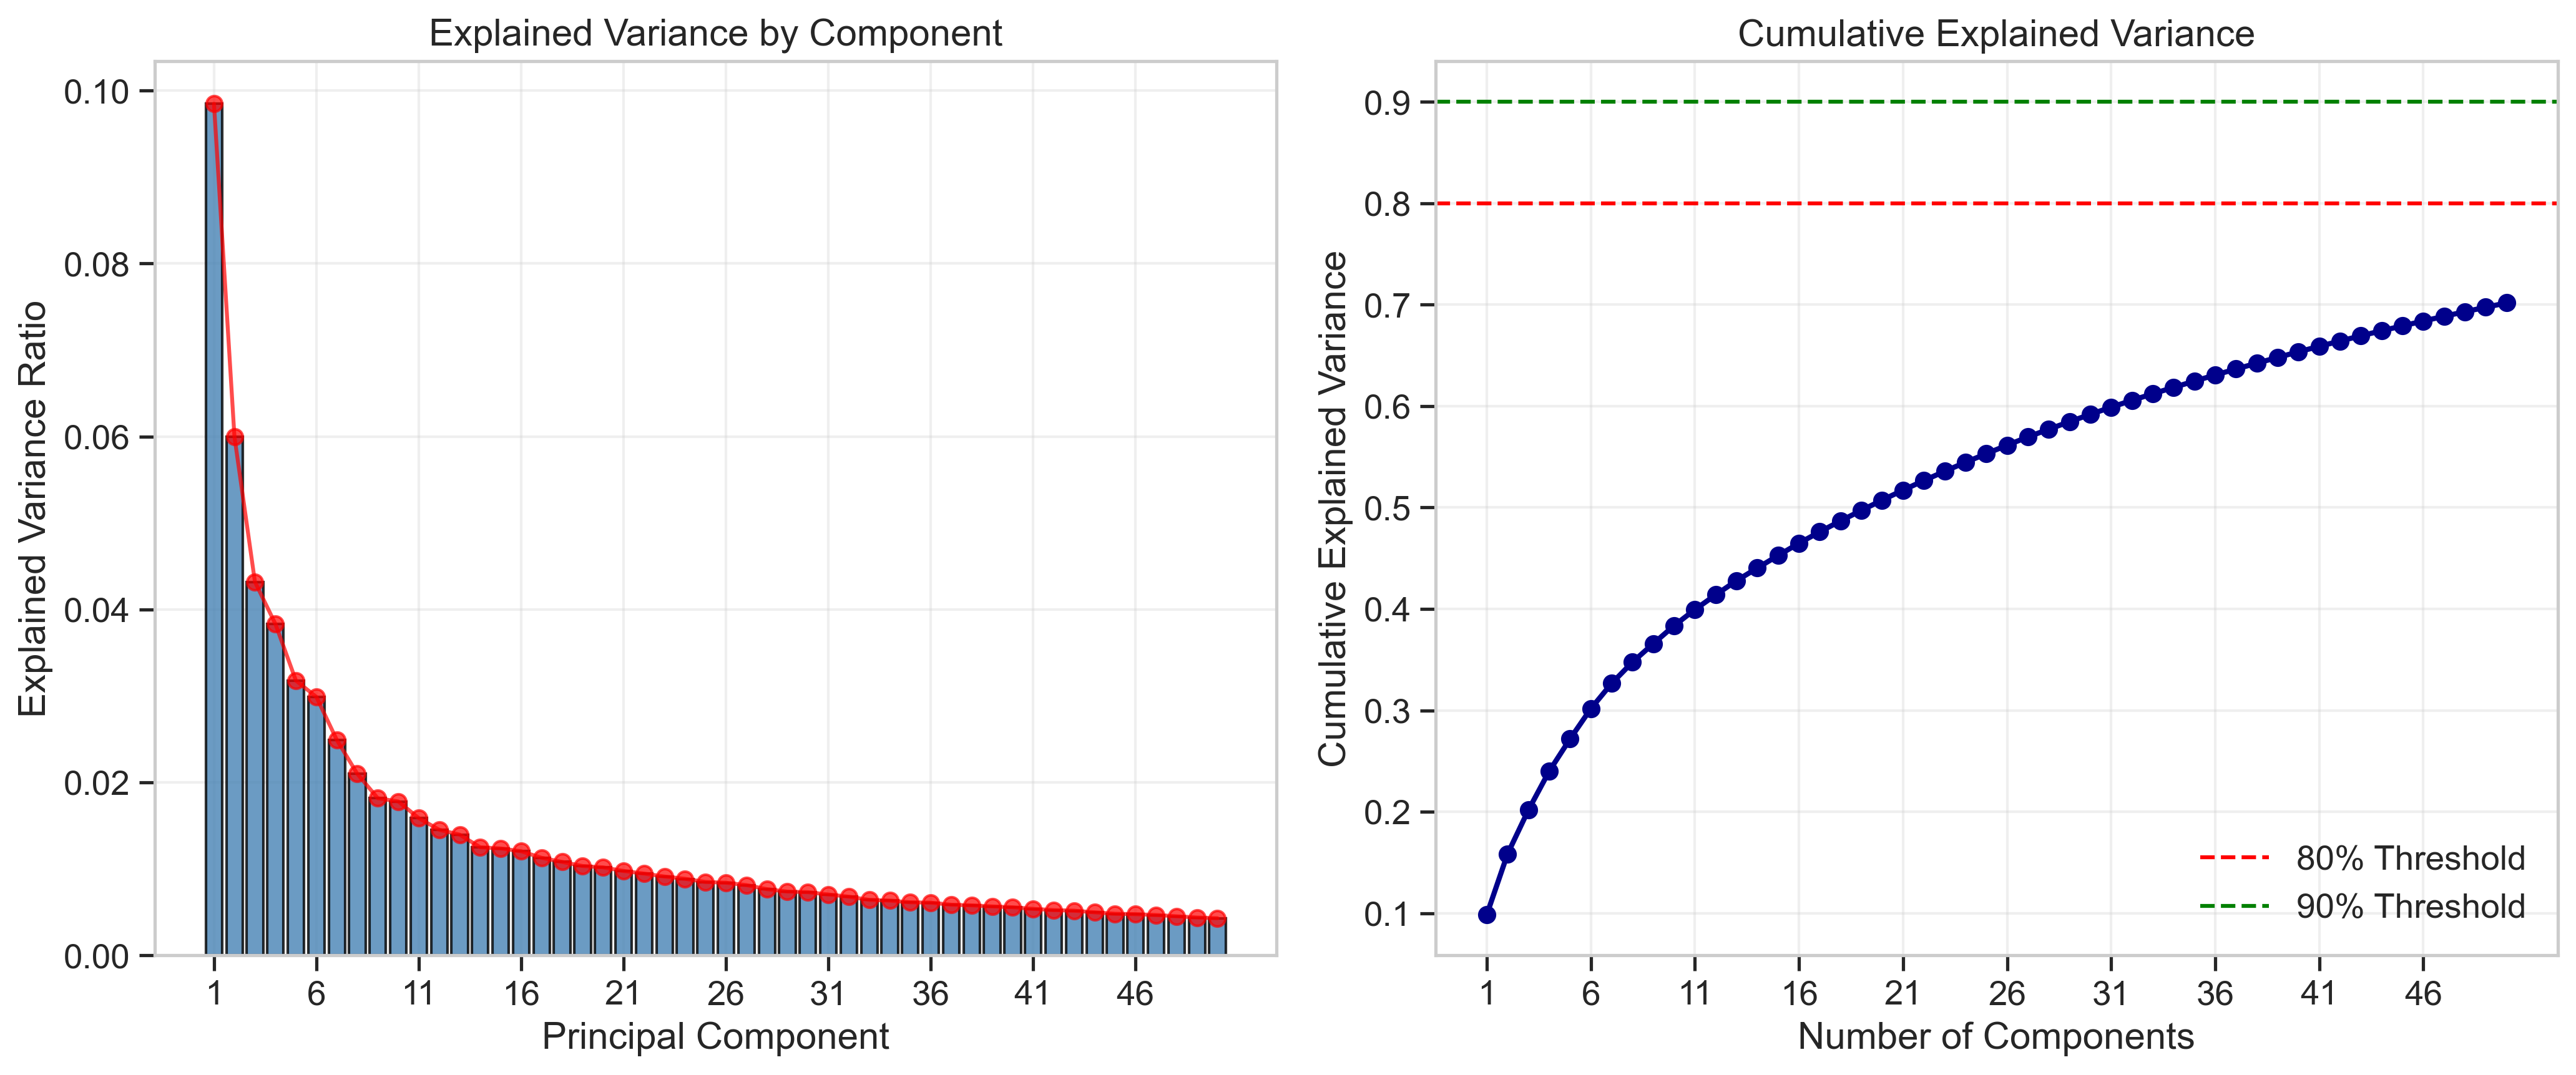
\includegraphics[width=0.9\textwidth]{figures/audio_features/pca_explained_variance.png}
  \caption{Explained variance by PCA components. Left: Individual variance contribution of each component. Right: Cumulative explained variance with 80\% and 90\% thresholds marked.}
  \label{fig:pca_variance}
\end{figure}

Analysis of the cumulative explained variance revealed that:
\begin{itemize}
    \item 82 principal components are sufficient to explain 80\% of the variance
    \item 146 components are needed to explain 90\% of the variance
\end{itemize}

This represents a significant dimensionality reduction (from 942 to 82 dimensions, or 91.3\% reduction) while maintaining most of the information content. The reduced feature set was used for subsequent clustering analysis.

\subsection{Feature Importance}

To understand which features contribute most to the principal components, the feature loadings for the top three components were analyzed.

\begin{figure}[H]
  \centering
  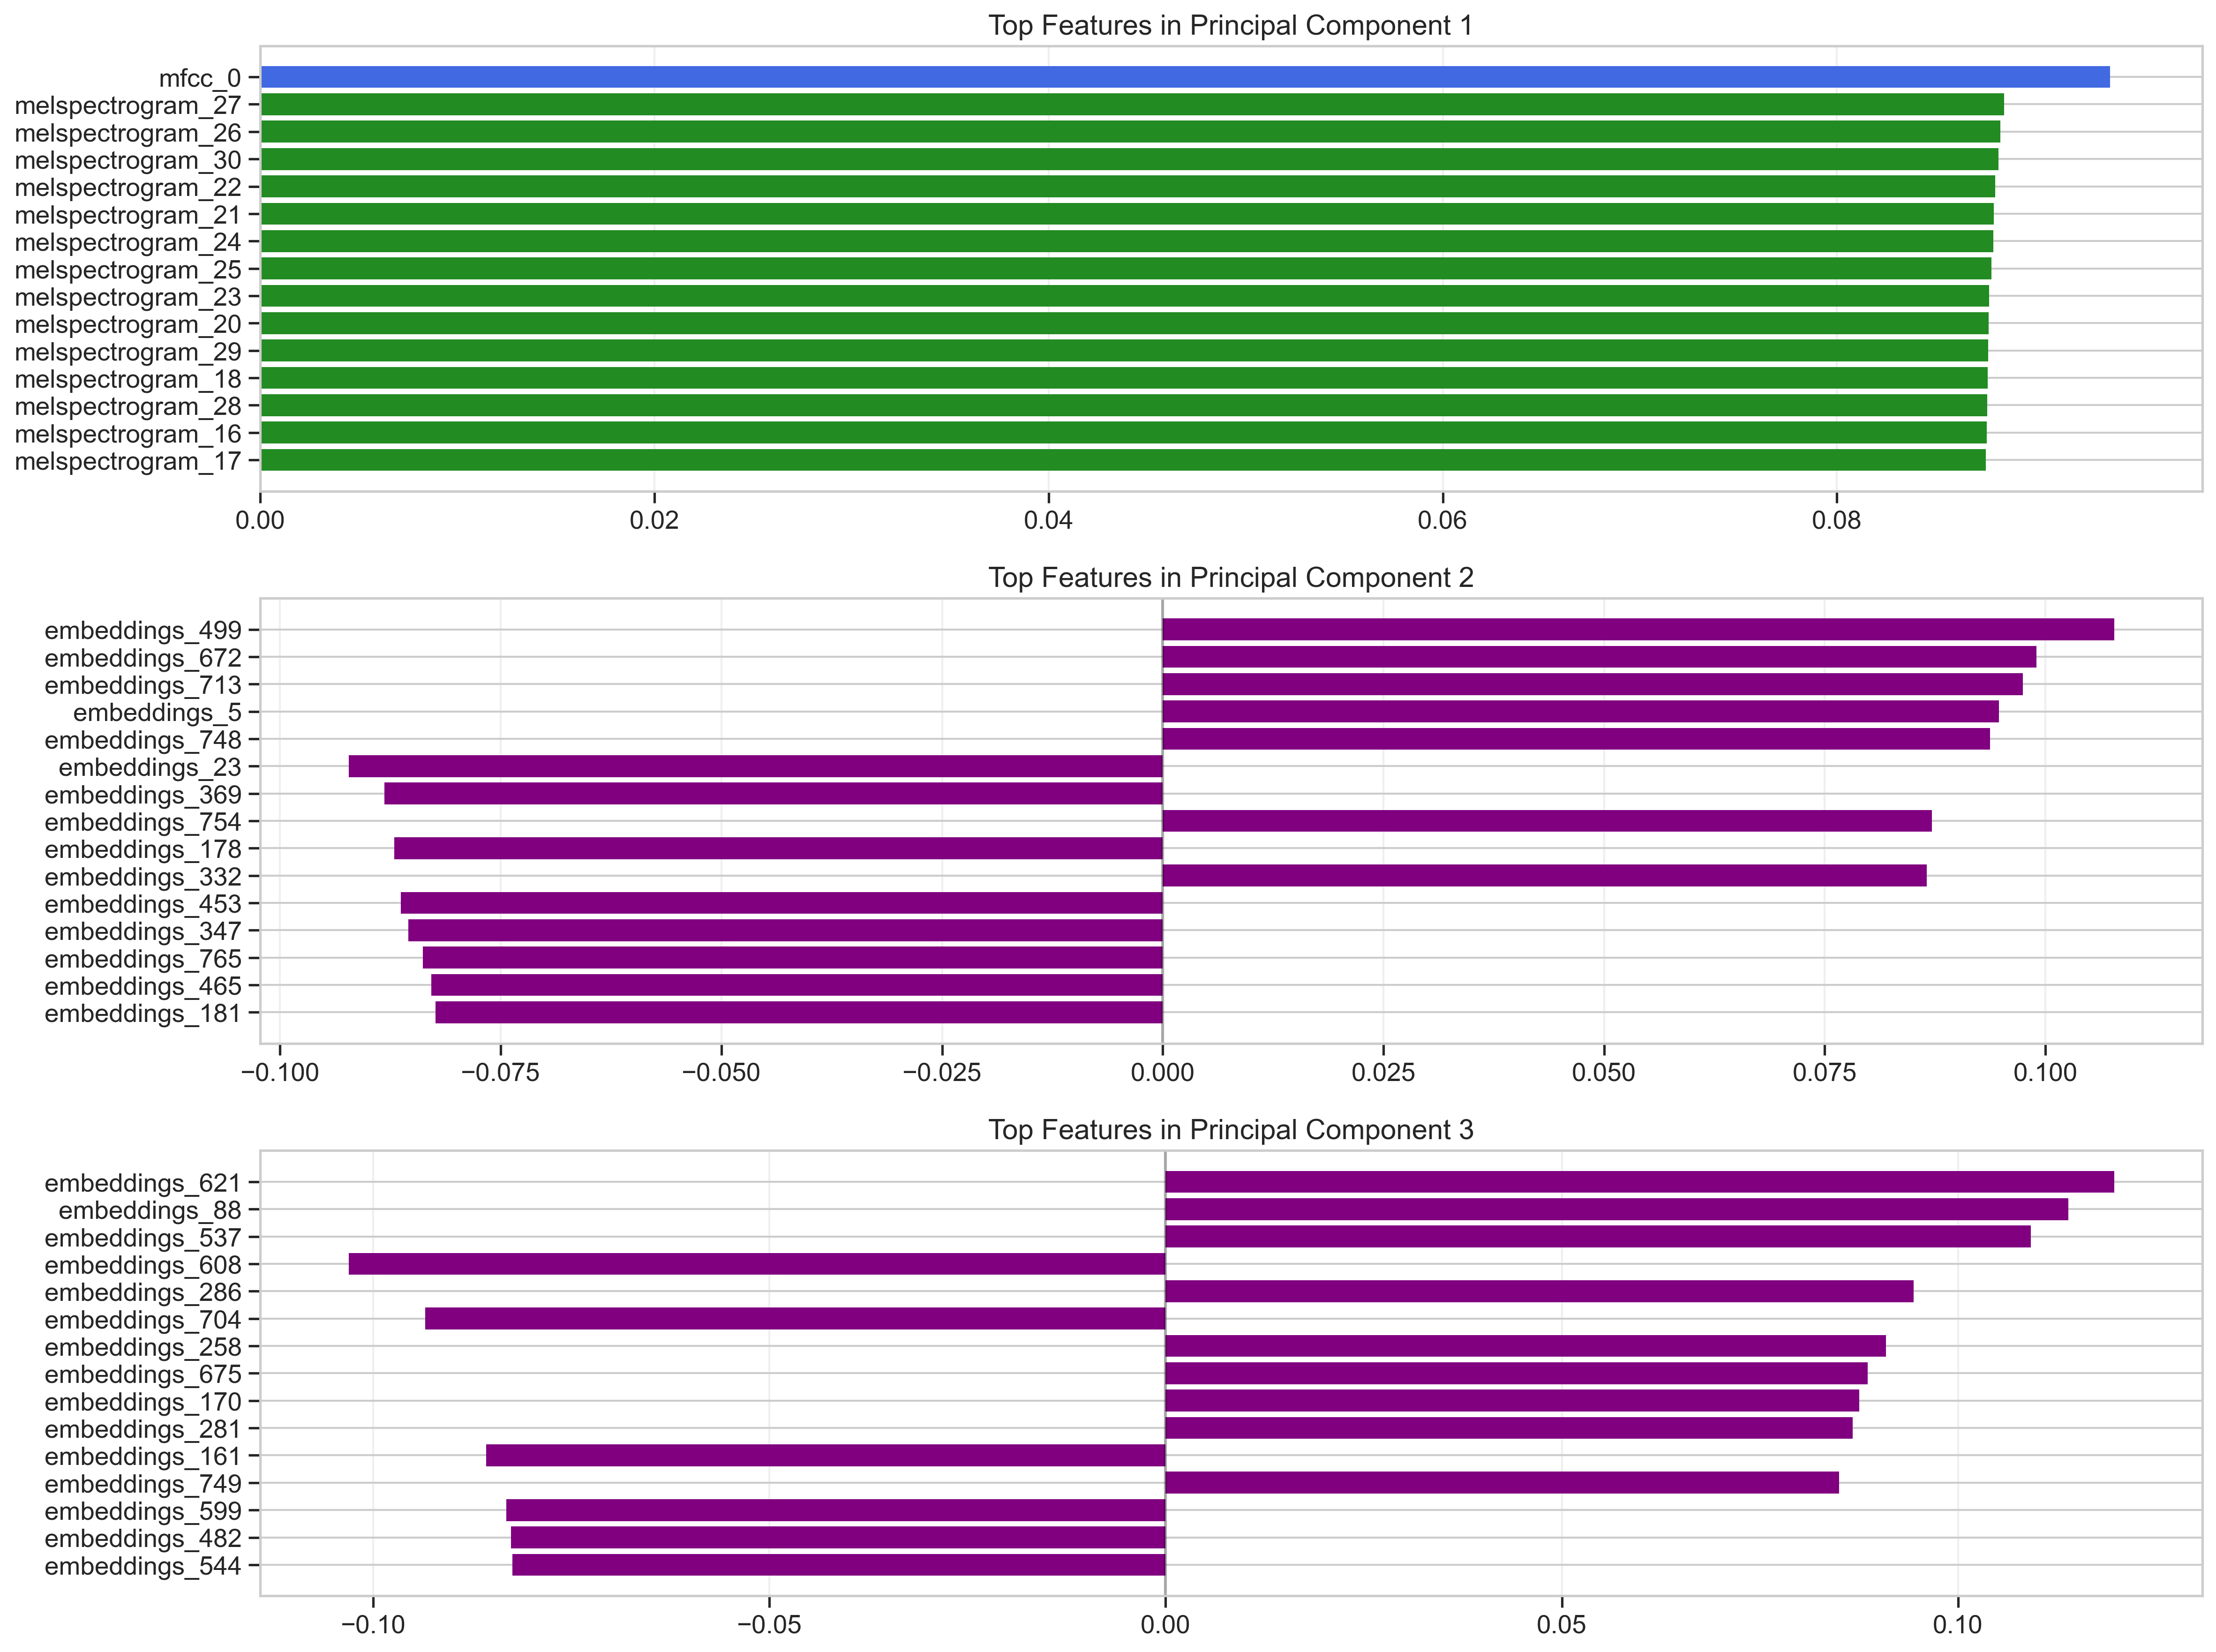
\includegraphics[width=0.9\textwidth]{figures/audio_features/feature_importance.png}
  \caption{Top 15 features contributing to the first three principal components, showing the relative importance of different feature types.}
  \label{fig:feature_importance}
\end{figure}

The analysis revealed:
\begin{itemize}
    \item \textbf{First principal component}: Dominated by Mel spectrogram features with MFCC\_0 (the DC component) having the highest loading. This suggests that energy distribution across frequency bands is the most significant factor for distinguishing audio signals.
    
    \item \textbf{Second and third principal components}: Heavily influenced by embedding features from the pre-trained neural network. These components likely capture higher-level semantic information about the audio content.
\end{itemize}

Across the top three components, the most important feature types were:
\begin{itemize}
    \item Embeddings: 30 occurrences
    \item Mel spectrogram features: 14 occurrences
    \item MFCCs: 1 occurrence
\end{itemize}

This suggests that while traditional spectral features like MFCCs are valuable, the learned embeddings capture additional information that contributes significantly to the variance in the data.

\subsection{Clustering Analysis}

K-means clustering was applied to the dimensionally-reduced feature vectors to identify natural groupings in the audio data. To determine the optimal number of clusters, silhouette scores were calculated for different values of k.

\begin{figure}[H]
  \centering
  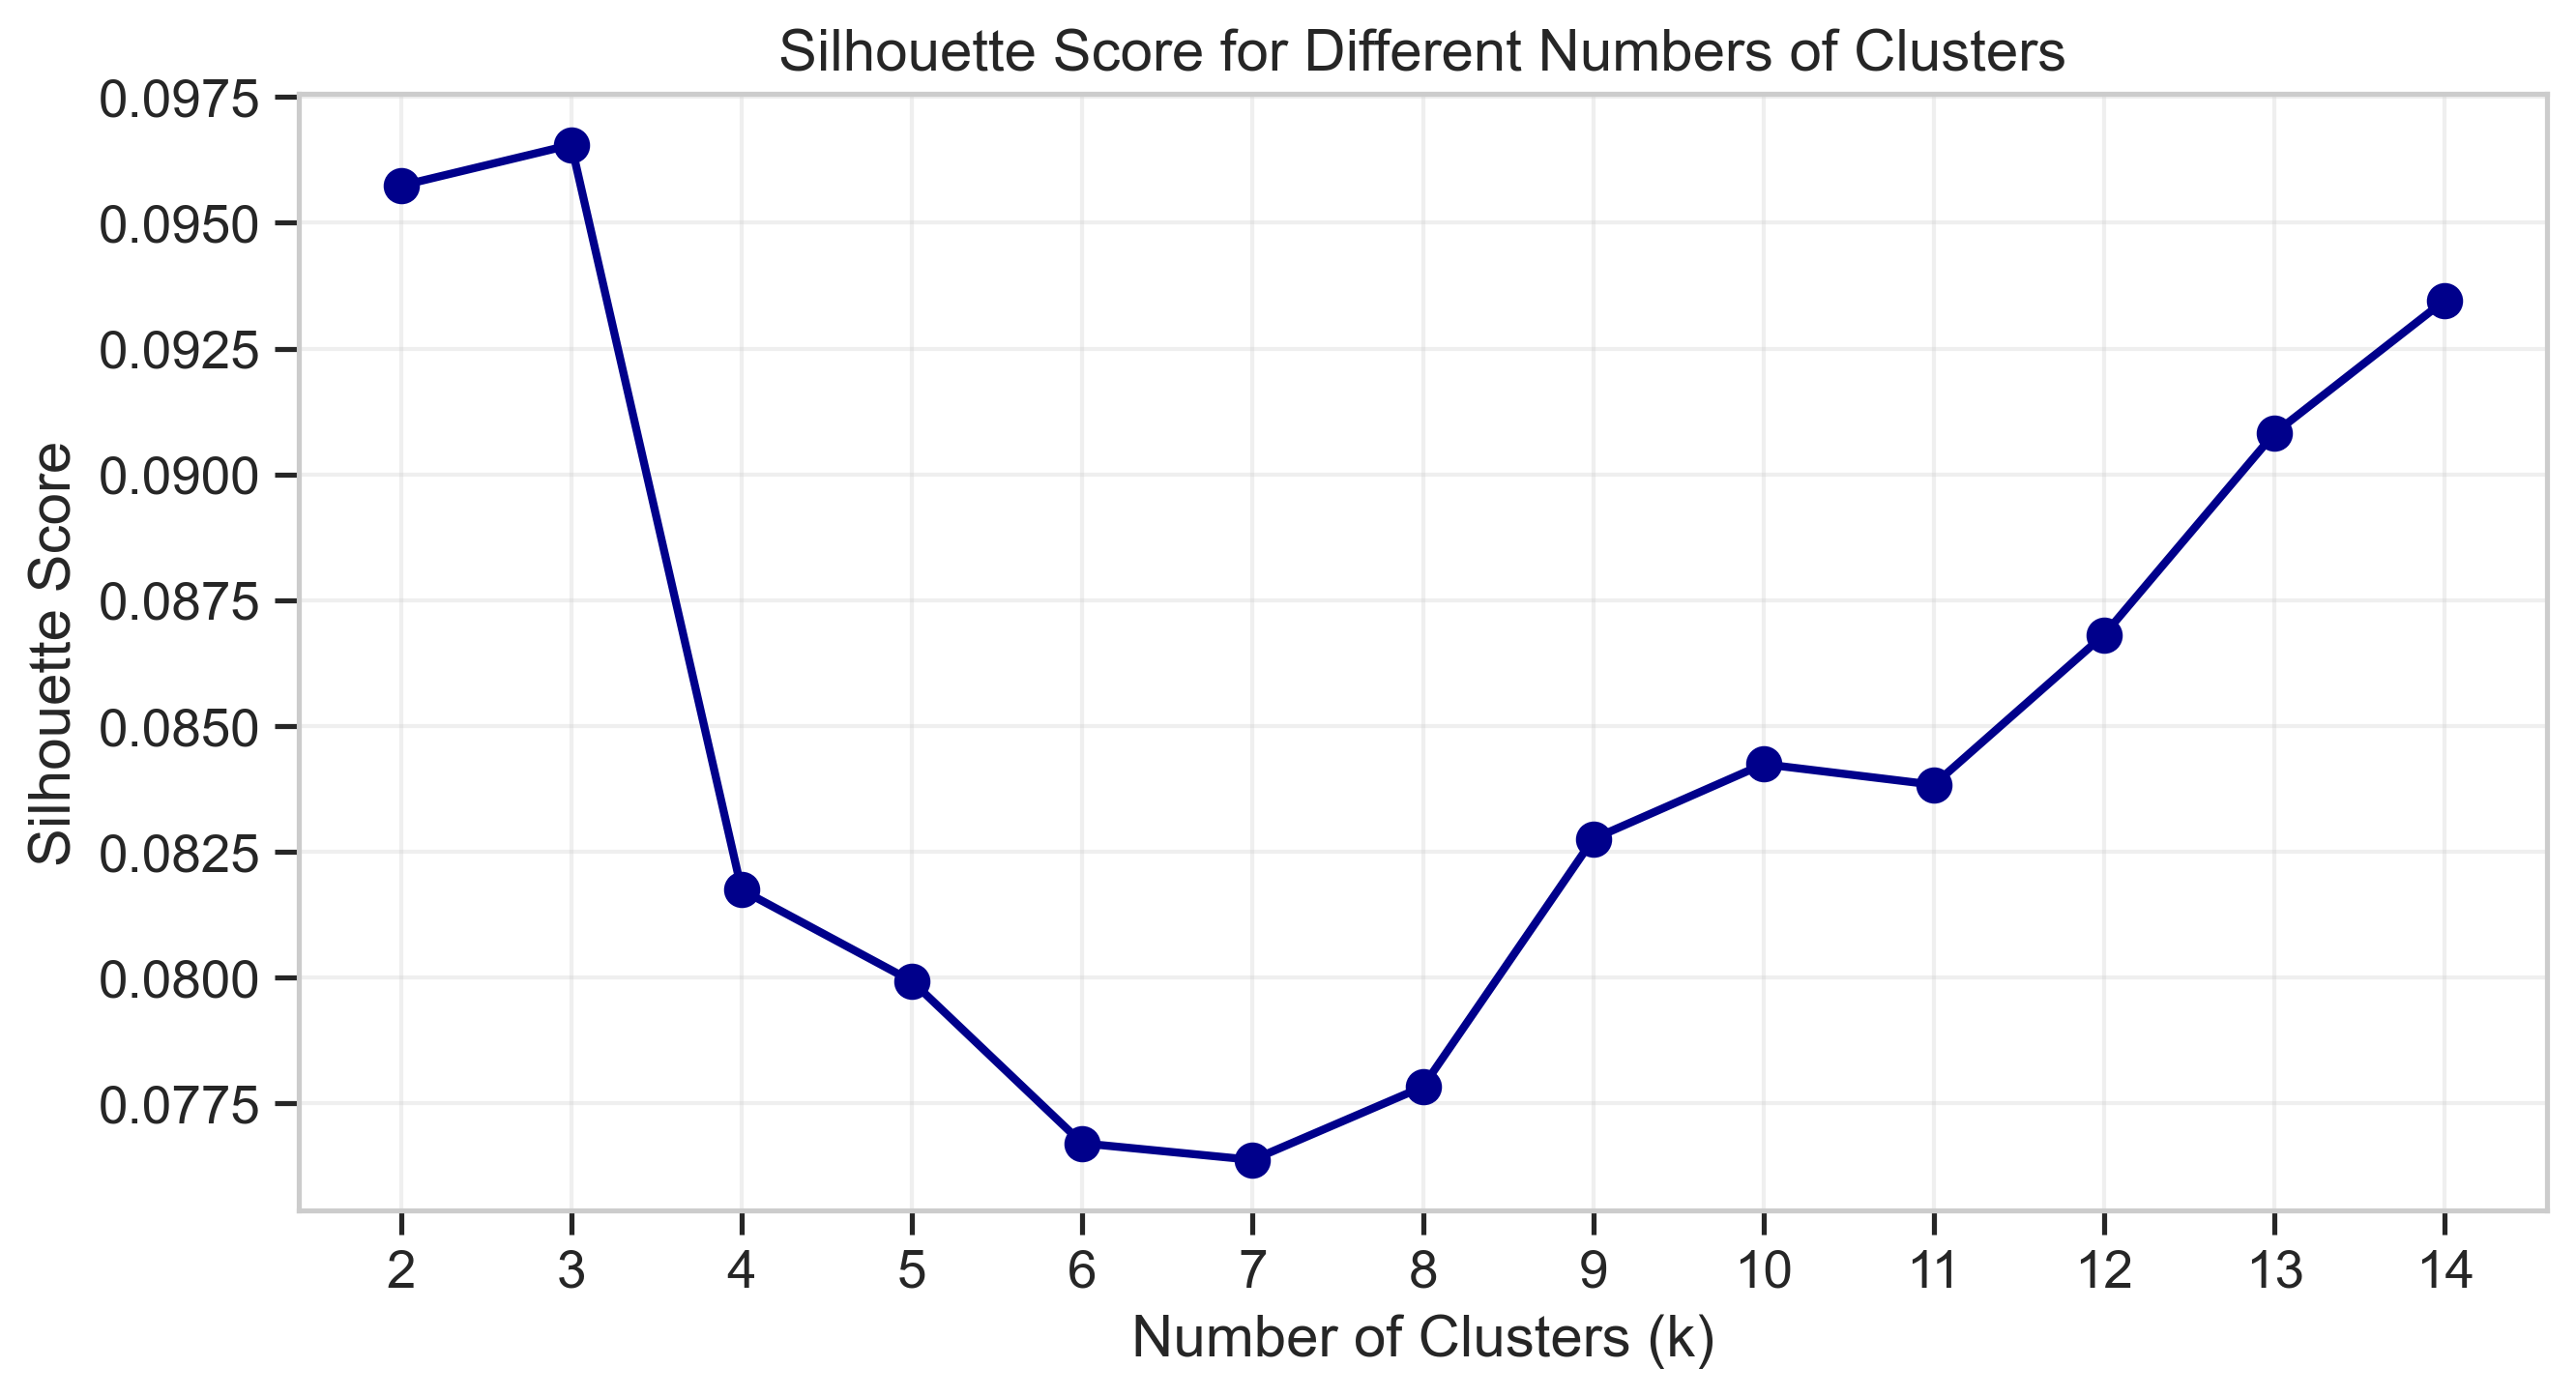
\includegraphics[width=0.8\textwidth]{figures/audio_features/silhouette_scores.png}
  \caption{Silhouette scores for different numbers of clusters (k), showing that k=3 provides the best cluster separation.}
  \label{fig:silhouette}
\end{figure}

The silhouette analysis indicated that 3 clusters provided the optimal balance between cluster separation and cohesion. The dataset was subsequently partitioned into these three clusters.

\begin{figure}[H]
  \centering
  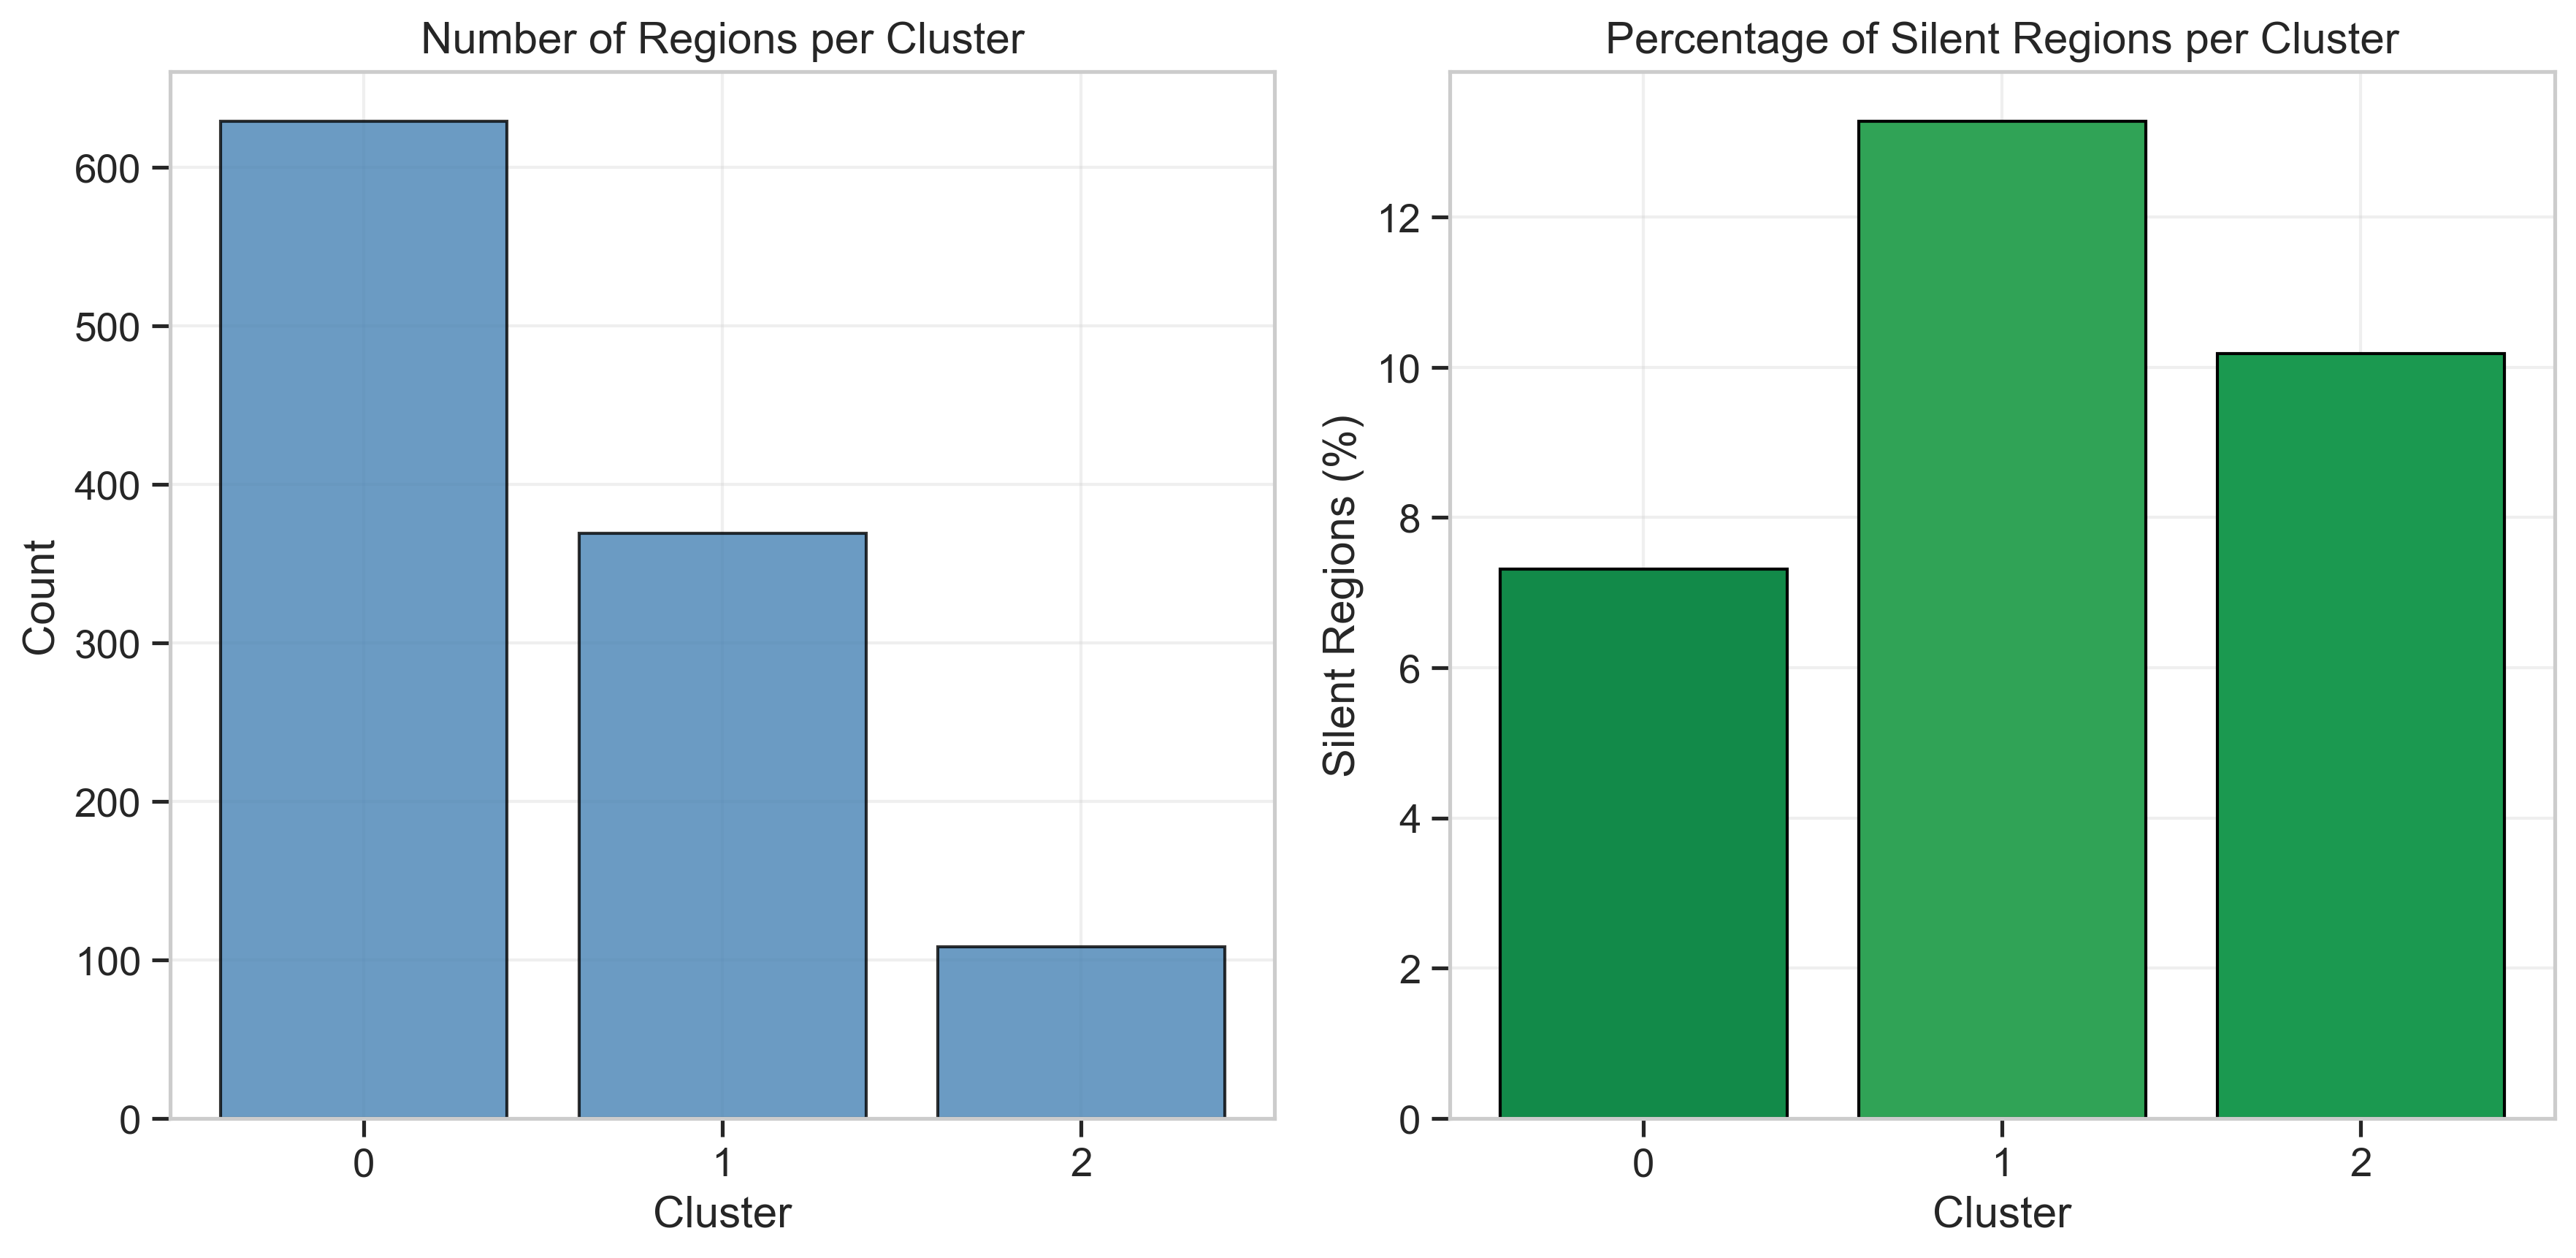
\includegraphics[width=0.9\textwidth]{figures/audio_features/cluster_composition.png}
  \caption{Left: Number of audio regions in each cluster. Right: Percentage of silent regions in each cluster.}
  \label{fig:cluster_comp}
\end{figure}

\subsection{Cluster Characteristics}

Analysis of the three clusters revealed distinct audio characteristics:

\begin{table}[H]
  \caption{Characteristics of the three audio feature clusters}
  \label{tab:cluster_chars}
  \centering
  \begin{tabular}{p{1.5cm}p{3cm}p{4cm}p{3cm}}
    \toprule
    \textbf{Cluster} & \textbf{Size \& Silent \%} & \textbf{Common Annotations} & \textbf{Audio Characteristics} \\
    \midrule
    Cluster 0 & 629 regions (56.9\%) \newline 7.3\% silent regions & Beeps, cat meows, pedestrian crossing sounds, metallic impacts & High embedding values, predominantly sharp, distinct sounds \\
    \midrule
    Cluster 1 & 369 regions (33.4\%) \newline 13.3\% silent regions & Insect buzzing, dog barking, bass drums, human vocalizations & Low embedding values, more sustained sounds with less tonal clarity \\
    \midrule
    Cluster 2 & 108 regions (9.8\%) \newline 10.2\% silent regions & Hihat sounds, guitar playing, rhythmic claps, alarm-like sounds & High embedding values, musical and rhythmic sounds \\
    \bottomrule
  \end{tabular}
\end{table}

Interestingly, silent regions were distributed across all three clusters rather than being concentrated in a single cluster. Cluster 1 had the highest percentage of silent regions (13.3\%), suggesting that this cluster might represent lower-energy or background sounds.

\subsection{Visualization of Audio Feature Space}

To visualize the high-dimensional feature space, t-Distributed Stochastic Neighbor Embedding (t-SNE) was applied to project the data into two dimensions while preserving local relationships.

\begin{figure}[H]
  \centering
  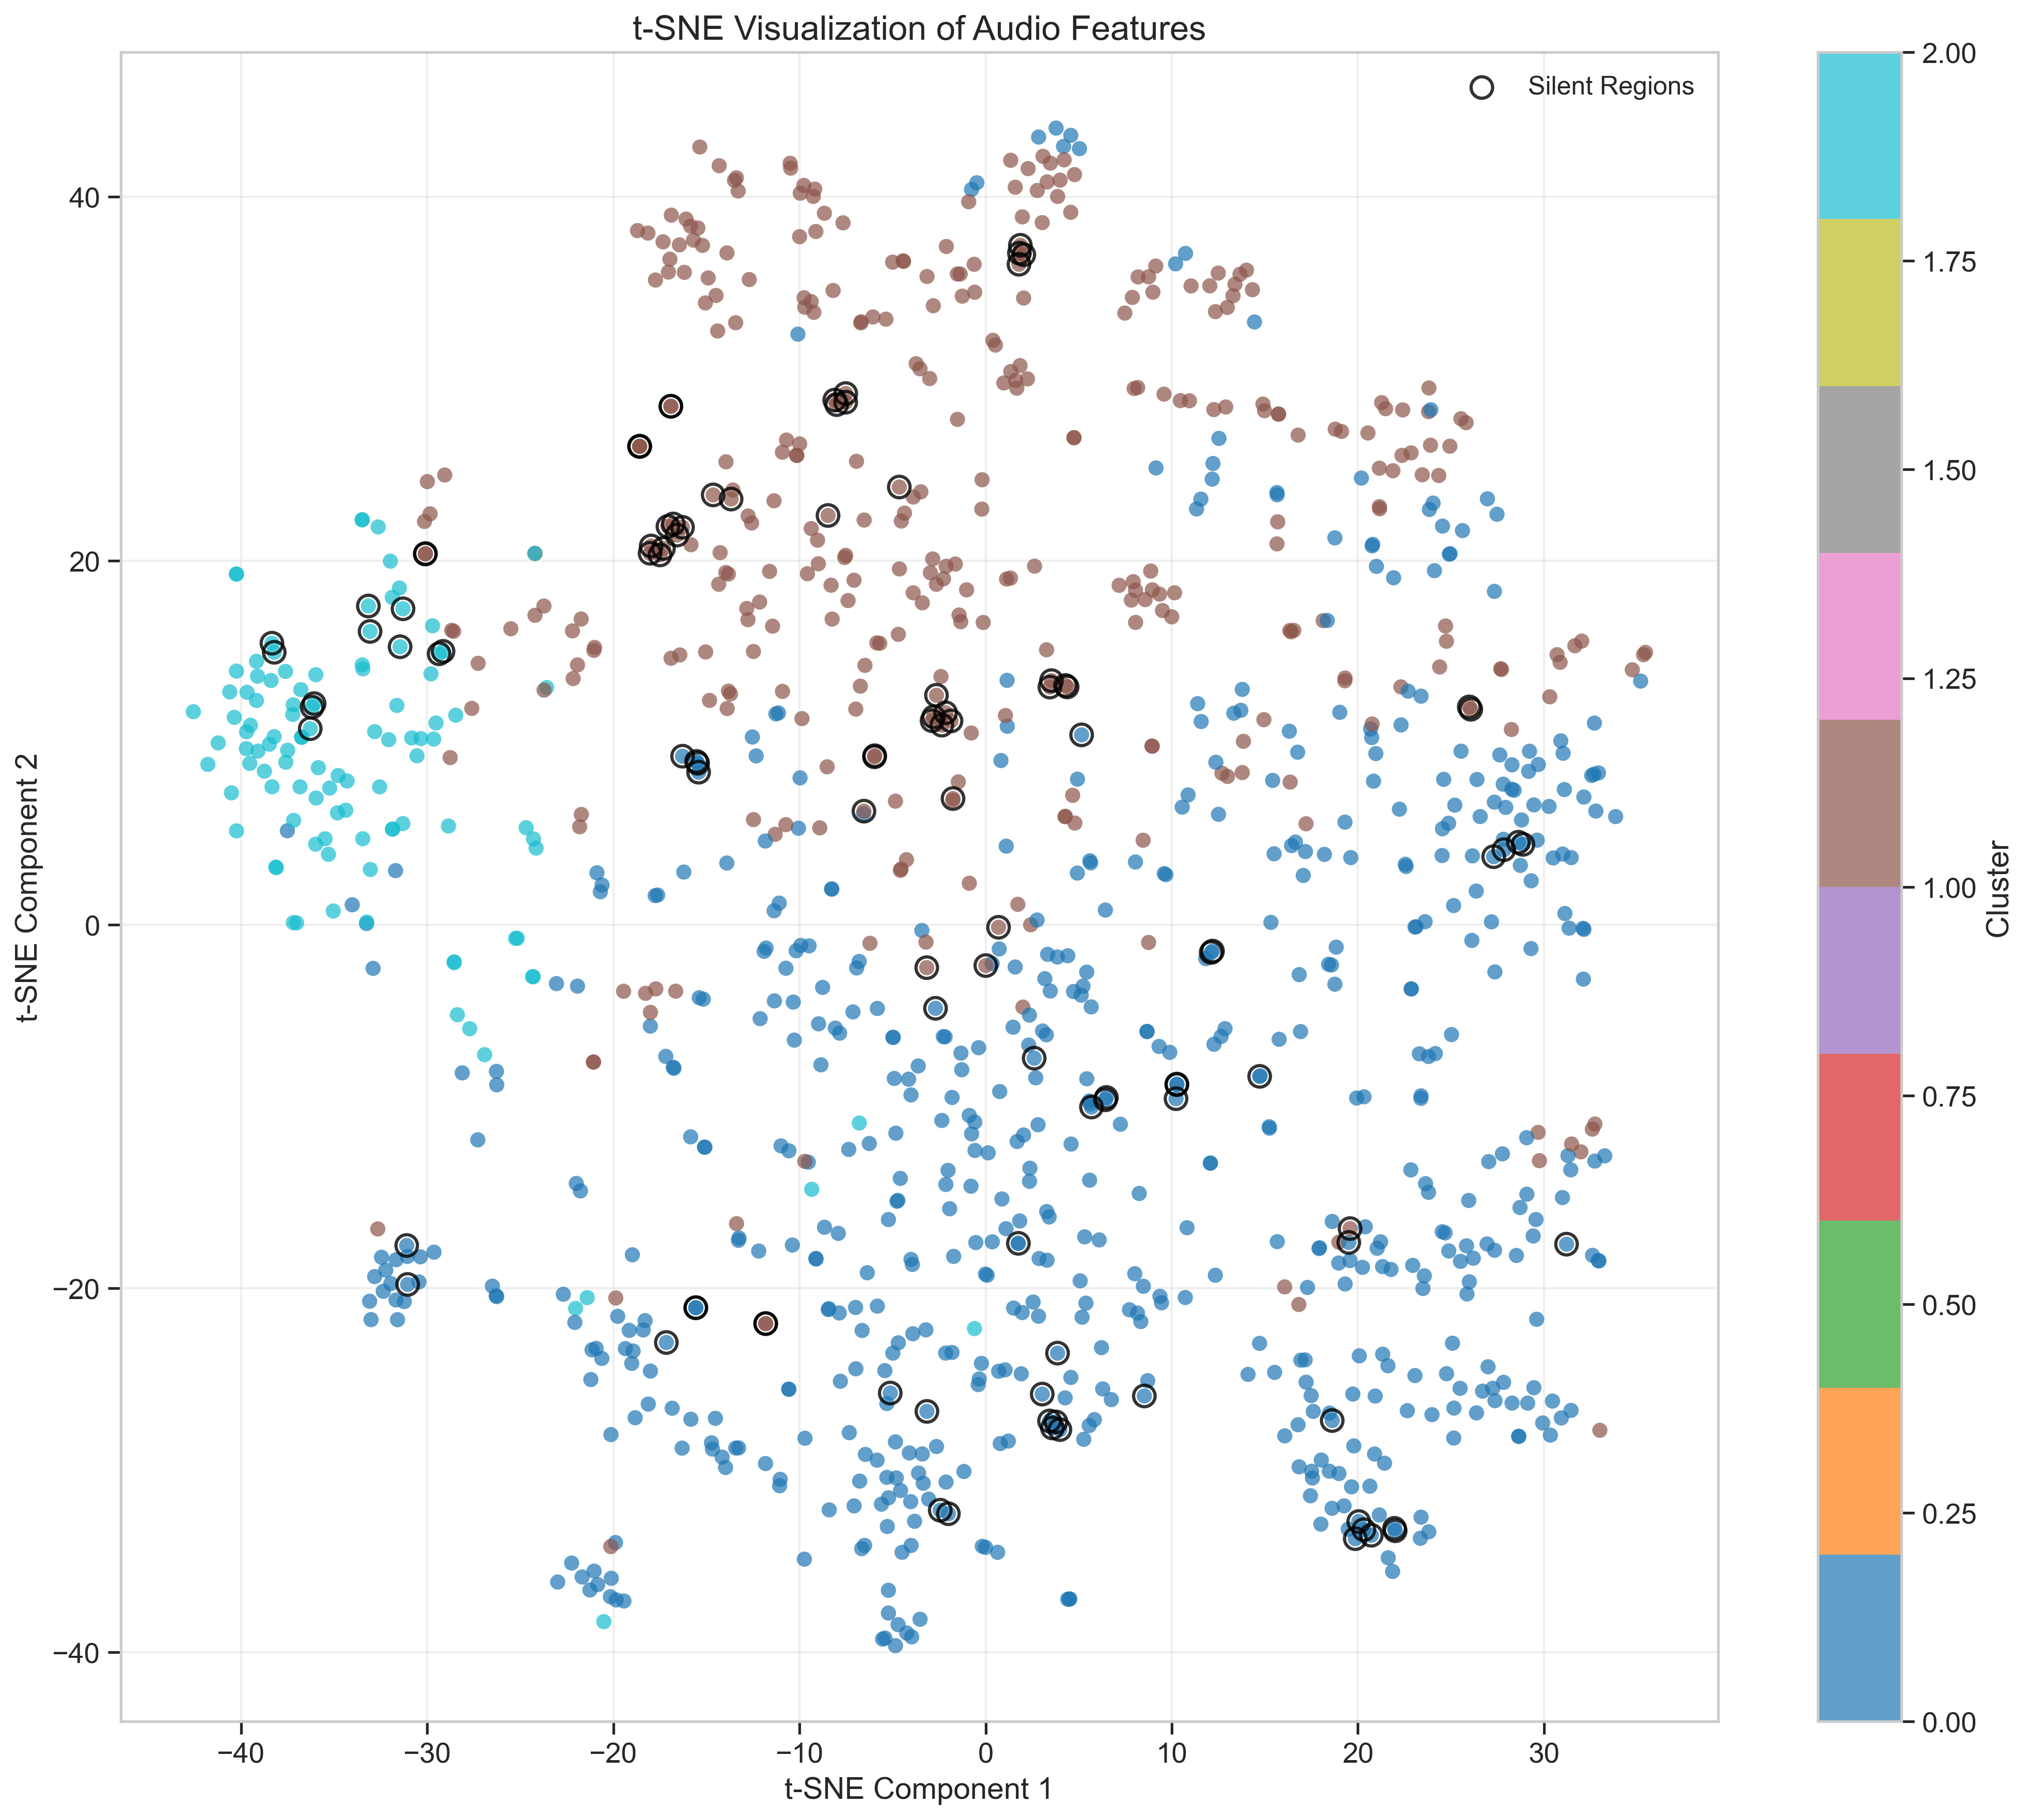
\includegraphics[width=0.8\textwidth]{figures/audio_features/tsne_visualization.png}
  \caption{t-SNE visualization of audio features colored by cluster assignment. Silent regions are highlighted with black circles.}
  \label{fig:tsne}
\end{figure}

The t-SNE visualization confirms the existence of distinct clusters in the audio feature space. However, it also shows that the boundaries between clusters are not always clear-cut, with some overlap between different sound types. Silent regions (marked with black circles) appear scattered throughout the feature space rather than forming their own distinct cluster, suggesting that the absence of sound is characterized differently depending on the context.

\section{Text Features}
\label{sec:text_features}

TODO: Analyze text features, cluster them to find meaningful groups, design labeling functions for dog and cat classes, and compare alignment between audio and text feature clusters.

\section{Conclusions}
\label{sec:conclusions}

TODO: Draw conclusions about the dataset's usefulness for training general-purpose sound event detectors and identify biases introduced during data collection and annotation.

\end{document}
